\documentclass[a4paper,12pt]{article}
\usepackage[hidelinks]{hyperref}
\usepackage[backend=bibtex]{biblatex}
\addbibresource{biblio.bib}
\usepackage{float}
\usepackage{graphicx}
\usepackage{listings}
\usepackage[utf8]{inputenc}
\usepackage{etoolbox}
\usepackage{fullpage}
\renewcommand*\contentsname{Indice}
\renewcommand*\figurename{Fig.}
\usepackage{setspace}
\usepackage{parskip}
\usepackage{subfigure}
\usepackage{amsmath}
\usepackage{blindtext}
\usepackage{enumitem}


\makeatletter
\patchcmd\l@section{%
  \nobreak\hfil\nobreak
}{%
  \nobreak
  \leaders\hbox{%
    $\m@th \mkern \@dotsep mu\hbox{.}\mkern \@dotsep mu$%
  }%
  \hfill
  \nobreak
}{}{\errmessage{\noexpand\l@section could not be patched}}
\makeatother

\setcounter{secnumdepth}{0}

\usepackage{fancyhdr}
\pagestyle{fancy}
\setlength{\headsep}{0.35in}
\let\MakeUppercase\relax

\setlength{\parindent}{2em}
\setlength{\parskip}{0.5em}
\renewcommand{\baselinestretch}{1.5}

\fancyhf{} 
\fancyfoot[C]{\thepage}

\frenchspacing

\begin{document}

\begin{titlepage}
\noindent
    \vspace*{5mm}
	\begin{minipage}[t]{0.15\textwidth}
	    \vspace*{5mm}
		\vspace{-3.5mm}{
\includegraphics[scale=1.8]{img/logo_bicocca.png}}
	\end{minipage}
	\hspace{1cm}
	\begin{minipage}[t]{0.9\textwidth}
	      \vspace*{5mm}
		{
			\setstretch{1.42}
			{\textsc{Università degli Studi di Milano - Bicocca} } \\
			\textbf{Scuola di Scienze} \\
			\textbf{Dipartimento di Informatica, Sistemistica e Comunicazione} \\
			\textbf{Corso di Laurea Magistrale in Informatica} \\
			\par
		}
	\end{minipage}
	
	\vspace{42mm}

\begin{center}
    {\LARGE{
	    	\setstretch{2}
            \textbf{
            	Sperimentazione Record Linkage \\ }
    }}        
\end{center}

\vspace{40mm}
	
	
	\begin{flushright}
		\setstretch{1.3}
		\large{Alberici Federico - 808058\\} 
		\large{Bettini Ivo Junior - 806878\\} 
		\large{Cocca Umberto - 807191\\} 
		\large{Traversa Silvia - 816435} 
	\end{flushright}
	
	\vspace{15mm}
	\begin{center}
		{\large{\bf Anno Accademico 2019 - 2020}}
	\end{center}


\renewcommand{\baselinestretch}{1.5}

\end{titlepage}

\tableofcontents

\newpage

\section{Ricerca preliminare} 

Il progetto che verrà esposto è consultabile alla seguente \href{https://github.com/ivemberg/Data_quality_experimentation}{\textbf{repository}}.

\subsection{Data Quality}

La consapevolezza del peso che dati di alta qualità hanno nel supportare decisioni informate e, viceversa, delle conseguenze disastrose cui dati inaccurati possono portare, è cresciuta di pari passo con il diffondersi delle fonti informative a disposizione delle organizzazioni, creando sempre più forte l’esigenza di una gestione adeguata della qualità dei dati aziendali. La ricerca sulla qualità dei dati è iniziata correttamente negli anni '90 e varie definizioni di ciò sono state date nel corso degli anni. \\

\noindent Un gruppo di ricerca del MIT, guidato dal professor Wang, ha definito la qualità dei dati come condizione per il loro utilizzo e ha proposto il loro giudizio dipendentemente dai consumatori finali. Allo stesso tempo, hanno definito una "dimensione della qualità dei dati" come un insieme di attributi che rappresentano un singolo aspetto o costrutto della qualità dei dati. \\

\noindent Sono necessarie tecniche di misurazione completa per consentire alle organizzazioni di valutare lo stato della qualità delle informazioni organizzative e monitorarne il miglioramento. \\

\noindent Ma cosa si intende quando si parla di qualità dei dati e come si misura? La qualità dei dati è una caratteristica che ha a che fare con la loro abilità di soddisfare le esigenze e le aspettative implicite o esplicite dell'utente. \\

\noindent Le best practices in questo ambito suggeriscono l’utilizzo di opportune metriche per la definizione e la misurazione della qualità dei dati. \\

\noindent Per quanto riguarda la definizione di metrica ci riferiamo alle definizioni all'interno dello standard ISO 9126-1 e framework ISM3:
\begin{itemize}
	\item una procedura (o metodo) di misurazione, cioè un algoritmo che prende l'elemento per misurare e lo associa a misura (sia esso valore ordinale o intervallo); 
	\item una corretta unità di misura (o scala), ovvero di dominio di valori restituiti dalla procedura di misurazione. In generale, è possibile associare diverse metriche a ciascuna dimensione di qualità;
\end{itemize} 
La data quality può essere espressa attraverso molteplici dimensioni. Le dimensioni dei dati nel modello relazionale sono:

\begin{itemize}
\item \textbf{Accuracy}: l'accuracy di un valore v è definita come vicinanza tra v e un valore v' considerato come corretta rappresentazione del fenomeno del mondo reale. Come metrica alfanumerici strutturati la metrica per l'accurancy sintattica è quella di adottare una funzione di distanza, per esempio la edit distance non normalizzata UED(v1, v2) che rappresenta il numero di inserimenti, cancellazioni e sostituzioni di simboli alfanumerici necessari per trasformare v1 in v2. Oppure abbiamo la edit distance normalizzata EDnorm(v1, v2) dove v1 e v2 sono valori nel dominio D, in cui il massimo numero di simboli è n:

\begin{center}
	\centering{$ EDnorm(v1, v2) = 1-ED(v1,v2)/n $}
\end{center}

\item \textbf{Completeness}: rappresenta la misura in cui i dati sono di succifiente ampiezza, profondità e portata a fini dell'attività in corso. La completezza nel modello relazionale può essere caratterizzata rispetto a presenza(assenza e significato di valori nulli, e validità di una delle due ipotesi dette assunzione a mondo aperto e assunzione a mondo chiuso. Data:
\begin{figure}[H]
	\centering
	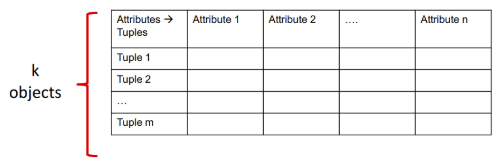
\includegraphics[width=0.8\linewidth]{img/table.png}
	\caption{\textit{tabella T che rappresenta un universo U di k oggetti }}
\end{figure}

Le metriche sono le seguenti:
\begin{figure}[H]
	\centering
	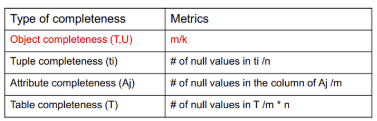
\includegraphics[width=0.8\linewidth]{img/metricheCompletezza.png}
	\caption{\textit{metriche principali completezza}}
\end{figure}

Le misure della completezza sono
\item \textbf{Currency}: è la dimensione che rappresenta la rapidità con cui i dati sono aggiornati rispetto a quando avviene il fenomeno. Per esempio il voto di un esame nella db studenti corsi-esami. Una prima misura della currency è il ritardo temporale tra il tempo $t_1$ dell'evento del mondo real che ha provocato la variazione del dato, e l'istante $t_2$ della sua registrazione nel sistema informativo. Questa misura è costosa perché in genere l'evento non è noto. Un'altra metrica è la currency come differenza tra tempo di arrivo alla organizzazione e tempo in cui è effettuato l'aggiornamento. Misurabile se c'è un log degli arrivi degli update.

\item \textbf{Tempestività}: misura quanto i dati sono aggiornati rispetto a un processo che li utilizza. La tempestività, al contrario della currency, è dipendente dal processo, ed è associata al momento temporale in cui deve essere disponibile per il processo che utilizza il dato.
\item \textbf{Consistency}: assume due significati uno legato alla consistenza dei dati con i vincoli d'integrità definiti sullo schema e un altro legato sulle diverse rappresentazioni di uno stesso oggetto della realtà presenti nella base di dati.
\end{itemize} 

\bigskip

\noindent Il punto focale rimane sempre il dominio sul quale si vuole effettuare un processo di miglioramento dei dati. In base alla finalità delle informazioni e alle caratteritiche dei loro consumatori l'attenzione si rivolge ad un sottoinsieme di tale metriche.\\

\noindent In tempi attuali, è emerso un altro tipo problema: i big data. Analisi e ricerca complete di standard di qualità e metodi di valutazione della qualità per questo tipo di informazioni attualmente è assente o non completa. Questo topic pone una serie di nuove sfide, dettate dalle caratteristiche intrinseche dei big data, riassumibili in quelle che sono chiamate "le 5 V":
\begin{itemize}
	\item \textbf{Volume}: ingente massa di informazioni, in crescita vertiginosa, che non è possibile raccogliere con tecnologie tradizionali;
	\item \textbf{Velocity}: i dati nascono e vengono acquisiti sempre più rapidamente, con necessità di analisi in tempo reale;
	\item \textbf{Variety}: differenti tipologie di dati disponibili, provenienti da un numero crescente di fonti eterogenee;
	\item \textbf{Veracity}: i dati devono essere affidabili, raccontare il vero;
	\item \textbf{Value}: abilità di trasformare una grande mole di dati in business.
\end{itemize}

\subsubsection{Metodologia Data Quality}

Il professor Batini definisce la metodologia di qualità dei dati come un insieme di linee guida e tecniche che, a partire dalle informazioni di input che descrivono un determinato contesto applicativo, ne deriva un processo razionale per valutare e migliorare la qualità dei dati \cite{10.1145/1541880.1541883}. Ci sono tre fasi principali per tale attività:
\begin{itemize}
\item \textbf{ricostruzione dello stato}, al fine di ottenere due informazioni contestuali, facoltative se sono già disponibili per l'uso;
\item \textbf{valutazione e misurazione}, misurazione della qualità lungo dimensioni della qualità pertinenti o valutazione, quando tali misurazioni vengono confrontate con i valori di riferimento;
\item \textbf{miglioramento}, attività che mirano per raggiungere nuovi obiettivi di qualità dei dati.
\end{itemize}

\subsubsection{Miglioramento}
Il miglioramento della qualità dei dati può essere effettuato attraverso strategie basate sui data-driven o su process-driven.

\noindent Nel primo caso, l'obiettivo è quello di migliorare la qualità dei dati direttamente modificando il valore del dato attraverso la comparazione con altri dati considerati di buona qualità. Le strategie più diffuse del data-driven sono quelle di: 
\begin{itemize}
	\item \textbf{acquisizione del nuovo dato}, che migliora il dato acquisendo dato di alta qualità per rimpiazzare il valore che causa proprlemi di qualità
	\item \textbf{record linkage}, che compara i dataset con valori sporchi con una fonte di dati di certificata, identificando tuple nei due dataset che potrebbero rappresentare lo stesso oggetto nel mondo reale;
	\item \textbf{affidabilità della fonte}, seleziona le origini dei dati sulla base della qualità delle fonti.
\end{itemize}
Nel process-driven l'obiettivo è quello di migliorare la qualità ridisegnando i processi che creano o modificano i dati, cioè andata a risolvere il problema alla radice. Le strategie più diffuse del process-driven sono quelle di: 
\begin{itemize}
	\item \textbf{processo di controllo}, che inserisce verifiche e procedure di controllo nel processo di produzione dei dati quando i dati sono creati, aggiornati o nuovi insieme dei dati sono accessibili dal processo.
	\item \textbf{ridisegnamento del processo}, per rimuovere le causa della qualità scarsa
\end{itemize}

\noindent Nel caso del nostro progetto, non abbiamo adottato strategie di process-driven perché non abbiamo un'applicazione che esegue il CRUD sui dati, ma abbiamo un insieme di txt che rappresentano delle istantanee di diversi datasets che indicano lo stesso concetto, realizzati in differenti istanti.

\subsubsection{Standardizzazione}

Questo processo, chiamato anche \textit{normalizzazione}, sostituisce o integra i valori dei dati con i valori corrispondenti conformi allo standard (ad esempio le abbreviazioni vengono sostituite con i nomi completi corrispondenti)

\subsubsection{Comparazione stringhe}

Gli errori tipografici rendono impossibile confrontare esattamente tra di loro le stinghe.  Per poter fare ciò, quindi, serve una funzione che cerca di trovare un punto di accordo tra i dati. Ci sono stati diversi tentativi di fornire questa funzione:

\begin{itemize}
\item Jaro \cite{census/jaro76} nel 1976 ha proposto un comparatore di stringhe che tiene conto di inserimenti, eliminazioni e trasposizioni necessarie per abbinare le due stringhe;
\item Winkler \cite{winkler90} nel 1990 ha proposto una variante della distanza Jaro (Jaro-Winkler);
\item la distanza q-gram conta il numero di q caratteri consecutivi che concordano tra due corde;
\item la distanza di edit classica, che conta il numero di operazioni (inserimenti, eliminazioni, modi cazioni) necessarie per abbinare le due stringhe
\end{itemize}

\subsection{Record Linkage}

Il record linkage (conosciuto anche come data matching) è l'operazione che consiste nel trovare "records" che si riferiscono alla stessa entità, in dataset presi da differenti risorse (come ad esempio file, libri, siti e database). \\

\noindent Questa operazione diventa necessaria quando vogliamo unire dei dataset differenti basati su dati simili che potrebbero avere o non avere lo stesso identificativo. \\

\noindent L'idea moderna di record linkage nasce alla fine degli anni cinquanta e viene formalizzata qualche tempo dopo da Ivan Fellegi e Alan Sunter \cite{fellegi69} che, attraverso il loro lavoro, hanno dimostrato che le regole di decisione probabilistiche sono ottimali quando i dati che vengono confrontati sono condizionatamente indipendenti. \\

\noindent A partire dalla fine degli anni novanta, differenti tecniche di machine learning sono state sviluppate per poter capire, con condizioni favorevoli, la probabilità condizionata richiesta dalla teoria Fellegi-Sunter. \\

\noindent Il record linkage può essere interamente eseguito senza l'aiuto di un computer, ma il motivo principale per cui esso viene utilizzato è perchè si vuole ridurre o eliminare le modifiche "fatte a mano" e per rendere più facile l'ottenimento del risultato. \\

\noindent Il record linkage si divide generalmente nei seguenti step:
\begin{enumerate}
\item vengono dati in input dei dataset;
\item viene definito uno spazio iniziale di ricerca;
\item si cerca di ridurre lo spazio di ricerca tramite un processo di "blocking" ;
\item viene definito lo spazio ridotto di ricerca;
\item vengono comparati i dati e viene presa una decisione;
\item vengono definitie le regole di matching, possibile matching o non-match;
\item secondo le regole definite viene generato il dataset di output.
\end{enumerate}

\begin{figure}[H]
	\centering
	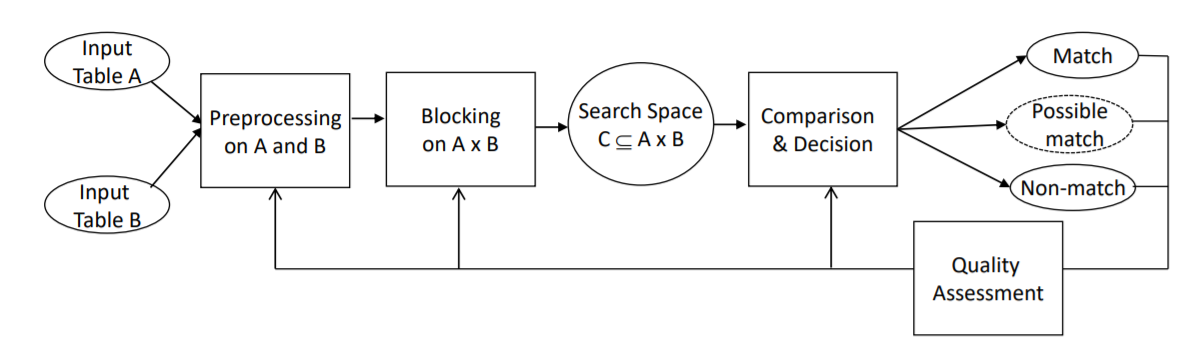
\includegraphics[width=0.8\linewidth]{img/recordlinkage.png}
	\caption{\textit{Step principali del record linkage}}
\end{figure}

\newpage
\subsubsection{Metodologie record linkage}

\begin{description}[align=left]
	\item[Data preprocessing] Il record linkage è molto sensibile alla qualità dei dati che devono essere collegati, quindi idealmente prima di svolgere questa operazione ogni dataset deve essere controllato affinche la qualità sia delle migliori. Avvengono delle operazioni di standardizzazione, che consistono nel trasformare i dati o procedure più complesse, come ad esempio la tokenizzazione.
	\item[Entity resolution] L'entity resolution è un processo di operazioni intelligenti che permettono alle organizzazioni di connettere i dati più disparati attraverso la possibilità di capire i matches tra le entità e le relazioni non ovvie fra i diversi dati.\\Essa analizza tutte le informazioni collegate ad una entità prese da diverse sorgenti e cerca, attraverso un calcolo probabilistico, di determinare quali entità sono collegate e quali collegamenti (non ovvi) esistono fra loro.
	\item[Deterministic record linkage] La metodologia più semplice di record linkage è chiamata "deterministica".\\Essa genera collegamenti basati sul numero di singoli identificatori che hanno una corrispondenza fra i dati dei dataset.\\Due record si dicono \textit{collegati} con una procedura di record linkage deterministico se tutti o alcuni degli identificatori sono identici.\\Questo metodo è una buona opzione se si stanno utilizzando dei dataset con delle entità che sono identificate da un id comune.
	\item[Probabilistic record linkage] Il record linkage probabilistico, chiamato anche \textit{fuzzy matching}, utilizza un approccio differente per poter collegare i dati. Viene tenuto conto di una gamma più ampia di potenziali identificatori, calcolando i pesi per ciascun identificatore in base alla sua capacità stimata di identificare correttamente una corrispondenza o una non corrispondenza. Questi pesi sono dunque usati per calcolare la probabilità che due dati registrati si riferiscano alla stessa entità.\\Le coppie di record con probabilità al di sopra di una determinata soglia sono considerate corrispondenze, viceversa le altre sono considerate non corrispondenze. Le coppie che rientrano tra queste due soglie sono considerate "possibili corrispondenze" e possono essere trattate di conseguenza (ad esempio, revisioni umane, collegate o non collegate, a seconda dei requisiti). Mentre il collegamento deterministico dei record richiede una serie di regole potenzialmente complesse da programmare in anticipo, i metodi probabilistici di collegamento dei record possono essere "addestrati" per funzionare bene con un intervento molto meno umano.
	\item[Machine learning] Negli ultimi anni, sono state utilizzate varie tecniche di apprendimento automatico per collegamento automatico. È stato riconosciuto che l'algoritmo classico per il collegamento probabilistico dei record sopra descritto è equivalente all'algoritmo Naive Bayes nel campo dell'apprendimento automatico, e utilizza la stessa assunzione dell'indipendenza delle sue caratteristiche (un presupposto che in genere non è vero).\\È possibile ottenere una maggiore precisione utilizzando varie altre tecniche di apprendimento automatico, incluso un percettrone a strato singolo. Insieme alle tecnologie distribuite, l'accuratezza e la scala per il collegamento dei record possono essere ulteriormente migliorate.	
\end{description}

\subsection{Tools}
Di seguito riportiamo i tools e le librerie che abbiamo utilizzato (o tentato di usare) durante il nostro progetto.

\subsubsection{Python Record Linkage Toolkit}
Python Record Linkage Toolkit è una libreria che permette di effettuare record linkage sia in una sola fonte di dati che in molteplici. Il toolkit fornisce la maggior parte degli strumenti necessari per il collegamento e la deduplicazione dei record.
Il package contiene metodi di indexing, come blocking e sorted neighborhood indexing, funzioni per il confronto con diverse misure di similarità possibili e diversi algoritmi di classificazione, sia supervisionati che non. 
Uno degli obiettivi principale è proprio creare un framework estendibile per il collegamento dei record, per fare questo il tool è in grado di:
\newpage
\begin{itemize}
\item pulire e standardizzare i dati
\item creare coppie di record con metodi di indicizzazione intelligente
\item confrontare i record con un gran numero di misure e di comparazione e somiglianza per diversi tipi di variabili
\item utilizzare diversi algoritmi di classificazione
\item valutare, attraverso strumenti comuni, i collegamenti dei record
\end{itemize} 

\noindent Per raggiungere l'obiettivo del nostro progetto è stato fondamentale poichè ci permette di svolgere tutte le operazioni del record linkage senza dover ricorrere all'utilizzo di ulteriori tool.

\subsubsection{Pandas}
Pandas è una libreria software scritta in linguaggio python che permette la manipolazione e l'analisi dei dati. L'obiettivo di questo tool è diventare il blocco di base di alto livello fondamentale per eseguire analisi dei dati reali. Inoltre, ha l'obiettivo più ampio di diventare lo strumento di analisi e manipolazione dei dati open source più potente e flessibile disponibile per qualsiasi linguaggio.\\

\noindent Questo tool è in grado di pulire, esplorare e elaborare i dati. In Pandas una tabella viene chiamata dataframe, ed è proprio grazie a questo tool che siamo riusciti  creare i due dataframe principali che poi utilizziamo nella fase di record linkage.

\subsubsection{Fuzzy Matcher}
Fuzzy Matcher è un pacchetto python che permette all'utente di collegare due dataframe pandas basati su uno o più campi in comune. Fuzzymatches usano la ricerca del testo completa sqlite3 per trovare dei match potenziali. Nonostante sia stato provato, non è stato poi incluso nel progetto poiché questa libreria non permette le stesse possibilità di sperimentazioni possibili con Record Linkage Toolkit, in quanto è più limitato.

\newpage
\section{Sperimentazione}

\subsection{Dataset}
Il dataset su cui sono stati effettuati gli esperimenti è un elenco di ristoranti di Manhattan, estratti settimanalmente da Gennaio a Marzo 2009 da 12 siti web. L'unico attributo comune in tutti i dataset è il nome del ristorante, informazioni aggiuntive (come l'indirizzo o il quartiere) non sono presenti in modo uniforme.
Insieme ai dataset era fornito un golden standard, ossia un elenco di 467 ristoranti rimossi da alcuni siti e il loro stato ("Y" = aperto, "N" = chiuso). Nell'ottica del progetto queste informazioni non sono risultate utili e per questo motivo non sono state sfruttate per analisi aggiuntive.

\subsection{Analisi dei dati}
I dati sono messi a disposizione in sette file di testo, uno per ogni settimana considerata, ciascuno contenente informazioni appartenenti a tutti i siti web. In totale sono presenti 215555 record, suddivisi come illustrato nella seguente tabella:
\begin{table}[H] \centering
\begin{tabular}{|l|l|}
\hline
\multicolumn{1}{|c|}{\textbf{file}} & \multicolumn{1}{c|}{\textbf{records}} \\ \hline
restaurants\_2009\_1\_22.txt & 30401 \\ \hline
restaurants\_2009\_1\_29.txt & 30775 \\ \hline
restaurants\_2009\_2\_05.txt & 30805 \\ \hline
restaurants\_2009\_2\_12.txt & 30863 \\ \hline
restaurants\_2009\_2\_19.txt & 30876 \\ \hline
restaurants\_2009\_2\_26.txt & 30898 \\ \hline
restaurants\_2009\_3\_12.txt & 30937 \\ \hline
\end{tabular}
\caption{Record presenti nei file txt forniti}
\end{table}

\noindent In particolare, per ogni ristorante è presente il seguente numero di record:

\begin{table}[H]\centering
\begin{tabular}{|c|c|}
\hline
\textbf{restaurant} & \textbf{records} \\ \hline
ActiveDiner & 6184 \\ \hline
DiningGuide & 814 \\ \hline
FoodBuzz & 2079 \\ \hline
MenuPages & 13143 \\ \hline
NewYork & 1774 \\ \hline
NYMag & 5124 \\ \hline
NYTimes & 3095 \\ \hline
OpenTable & 1539 \\ \hline
SavoryCities & 4536 \\ \hline
TasteSpace & 3635 \\ \hline
TimeOut & 14007 \\ \hline
VillageVoice & 2684 \\ \hline
\end{tabular}
\caption{Record per ristorante}
\end{table}

\noindent Sono presenti le seguenti informazioni: 
\begin{itemize}
\item \textbf{ActiveDiner}: nome ristorante, indirizzo, paese
\item \textbf{DiningGuide}: nome ristorante, indirizzo
\item \textbf{FoodBuzz}: nome ristorante, indirizzo, paese, codice paese, quartiere, tipo, costo
\item \textbf{MenuPages}:nome ristorante, indirizzo1, indirizzo2
\item \textbf{NewYork}: nome ristrorante
\item \textbf{NYMag}: nome ristorante, quartiere
\item \textbf{NYTimes}: nome ristorante, quartiere
\item \textbf{OpenTable}: nome ristorante, quartiere
\item \textbf{SavoryCities}: nome ristorante, indirizzo, quartiere
\item \textbf{TasteSpace}: nome ristorante, indirizzo, paese
\item \textbf{TimeOut}: nome ristorante, posizione, indirizzo1, indirizzo2, indirizzo3, quartiere, numero di telefono, tipo
\item \textbf{VillageVoice}: nome ristorante, indirizzo, quartiere
\end{itemize}

\noindent Possiamo notare che non sono presenti tutte le stesse informazioni in tutti i dataset, cosa che ci ha recato non pochi problema durante la fase di linkage. Per questo motivo il dataset "NewYork" non è stato utilizzato poichè non portava informazione utile.

\subsection{Data preprocessing} 
Una prima analisi mostra come le modalità di recupero dei dati da parte dell'autore abbiano generato dei dataset differenti per schema e per frammentazione verticale, anche sulle stesse fonti. Dunque, prima di applicare le tecniche di record linkage, i dati sono stati standardizzati, eseguendo operazioni di riallineamento dello schema, rimozione dei duplicati ed infine join dei dataset per fonte.\\

\noindent La fase di preprocessing, nella quale sono incluse la pulizia dei dati e la standardizzazione, sono importanti poiché potrebbero aumentare l'accuratezza del record linkage.\\
In dettaglio le fasi del preprocessing sono state: % PER FEDE: mettere esempi più precisi dei problemi trovati
\begin{enumerate}
	\item \textbf{Separazione e ragruppamento dei dati per fonte}.\\Ciò ha mostrato le differenze sullo schema, utilizzate nelle fasi successive per migliorare il raggruppamento dei dati.
	\item \textbf{Separazione dei dati per fonte e data}.\\Utilizzando regex ad hoc per ogni fonte i dati sono stati separati per fonte e data, con drop dei duplicati, standardizzazione dell'encoding del testo (da \textit{windows-1252} a \textit{UTF-8}) e formato csv.
	\item \textbf{Merge dei dataset per fonte}.\\I vari dataset risultanti dalla fase 2 sono stati riuniti per fonte con un join applicato su colonne definite a priori. 
	\item \textbf{Pulizia finale}.\\I dataset dunque sono stati ripuliti utilizzando delle funzioni specifiche per ogni fonte, con il compito di riallineare lo schema, rimuovere duplicati e caratteri superflui dai valori (es spazi e tabulazioni in testa e in coda, caratteri speciali ecc.).  
\end{enumerate}

\subsection{Google Maps}
Nei vari dataset le informazioni riguardanti l'indirizzo non erano riportare in maniera uniforme (es. \textit{Street} in un record e \textit{St.} in un altro), quindi abbiamo deciso di standardizzare questo parametro ricorrendo alle API di Google Maps.

\noindent Come prima cosa abbiammo creato una API key per poter dialogare con le 
\textbf{\href{https://console.cloud.google.com/google/maps-apis/overview?project=feisty-nectar-281812&folder=&organizationId=}{API di Google}}


\noindent Consultando la \href{https://developers.google.com/places/web-service/search}{documentazione} abbiamo individuato la funzione 
Text Search, la quale è molto simile alla funzione di autocompletamento presente su Google Maps e che quindi ci permette di ricavare indirizzo completi partendo da informazioni parziali.

\noindent Pertanto è stato costruito uno script che esegue una GET al seguente \href{https://maps.googleapis.com/maps/api/place/textsearch/json }{indirizzo}, passando come parametro la stringa \textit{address} del record del csv considerato. L'output ottenuto è un json, come si può osservare nel seguente esempio presente nella documentazione ufficiale.

% la si può prendere direttamente dal sito di google nella funzione textsearch PER UMBE CHE VUOL DIRE??
% https://console.cloud.google.com/google/maps-apis/overview?project=feisty-nectar-281812&folder=&organizationId=
\begin{figure}[H]
	\centering
	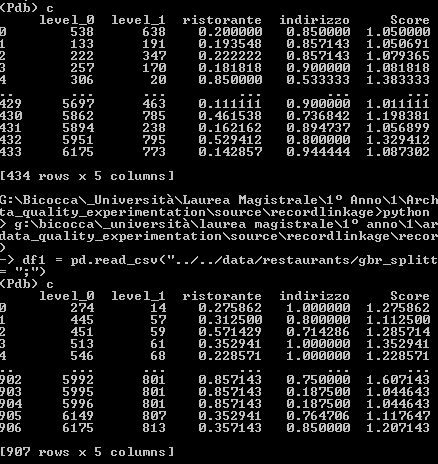
\includegraphics[width=0.8\linewidth]{img/img.png}
	\caption{\textit{Dati dopo il preprocessing di MenuPages}}
\end{figure}

\noindent Il campo da noi considerato è formatted\_address. In caso di indirizzo scritto male o con contenuto informativo ambiguo venivano restituiti più formatted\_address, pertanto si è deciso che se il numero di risultati ottenuto era maggiore di 5 allora non si è applicata tale trasformazione, poiché probabilmente non porterebbe reali benefici. Negli altri casi si è preso solo il primo risultato. 

\noindent Nello specifico,  dato che tutti i ristoranti sono a New York, abbiamo splittato la stringa recuperando solo la prima parte (fino alla prima virgola), in quanto l'informazione sulla città è superflua. 
 
Considerando l'esempio riportato nell'immagine sopra, da un indirizzo del tipo \textit{140 George St, The Rocks NSW 2000, Australia} manteniamo solo la parte \textit{140 George St}

\noindent In questo modo facendo i confronti il contenuto informativo era maggiore e non degradato da New york, NY , dati che sarebbero stati comuni a tutti.

\subsubsection{Risultati}
Nel caso di MenuPages, per esempio, inizialmente i dati erano presenti in un txt in questo formato ed erano uniti ai dati di altri siti web:\\
\begin{figure}[H]
\centering
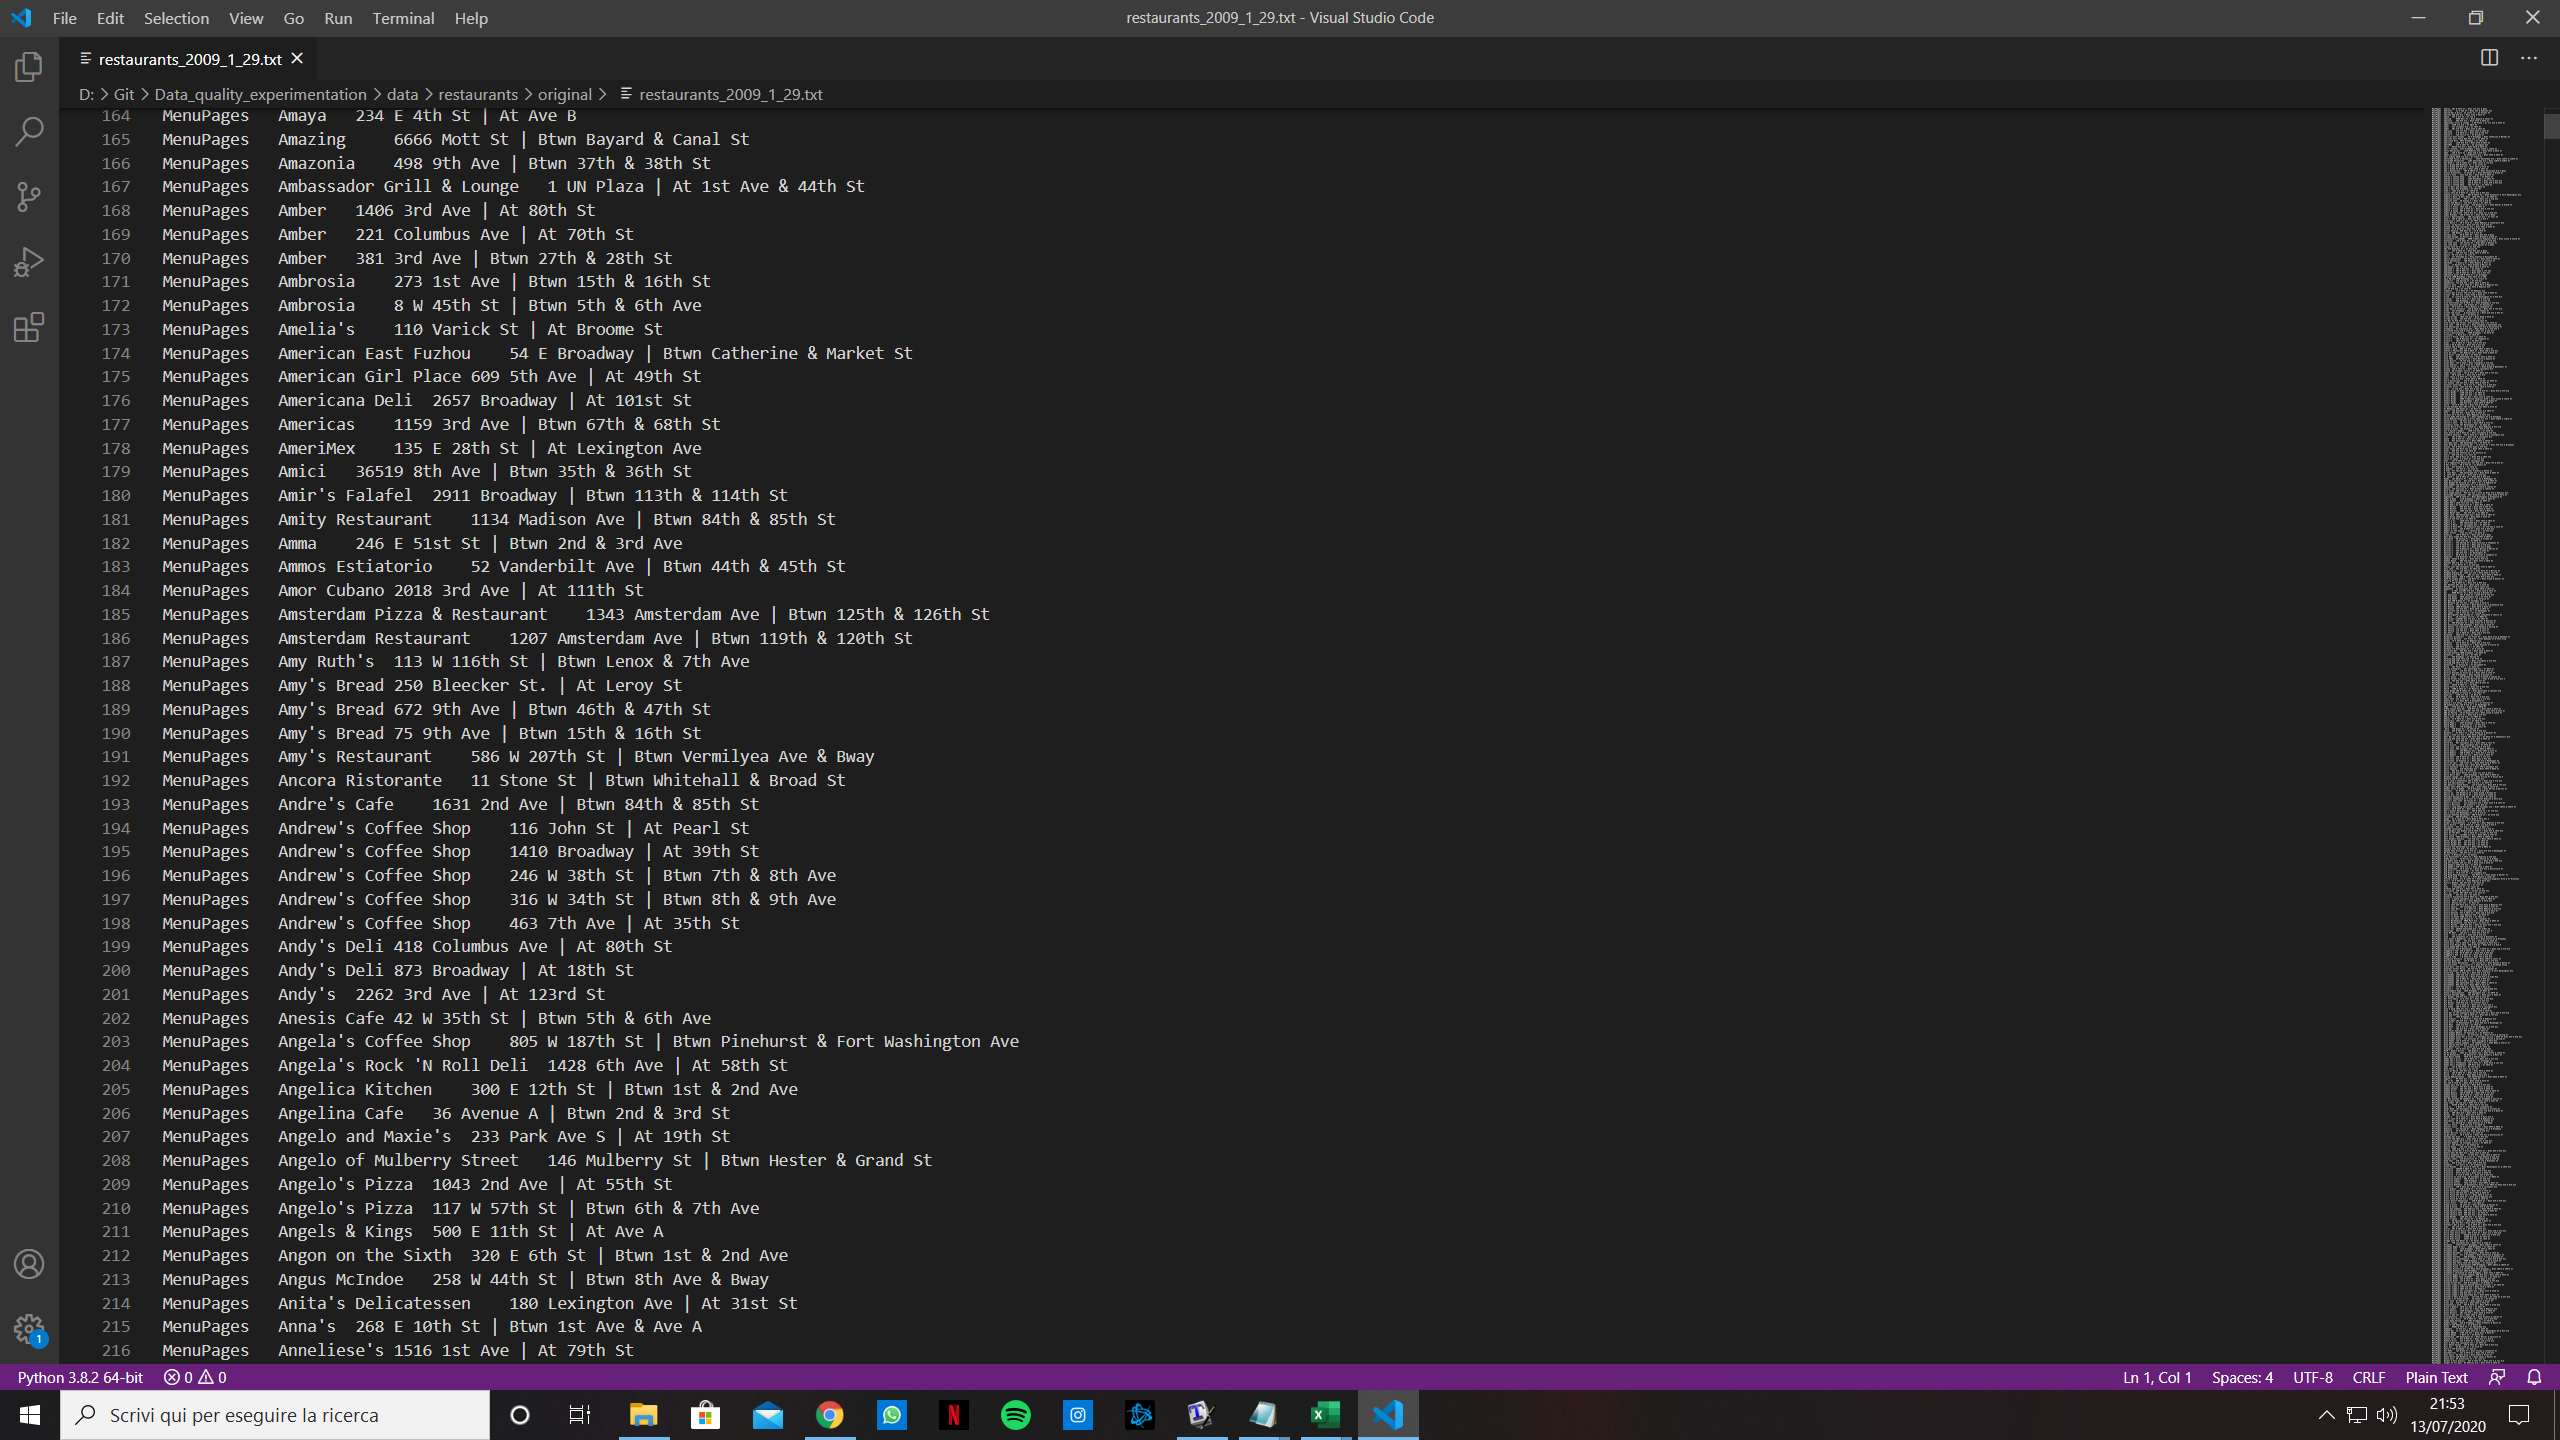
\includegraphics[width=0.9\linewidth]{img/original.png}
\caption{\textit{Dati di partenza di MenuPages}}
\end{figure}

\noindent A seguito del preprocessing invece otteniamo informazioni più chiare, aggiungendo l'informazione sull'indirizzo proveniente da Google come segue:\\

\begin{figure}[H]
\centering
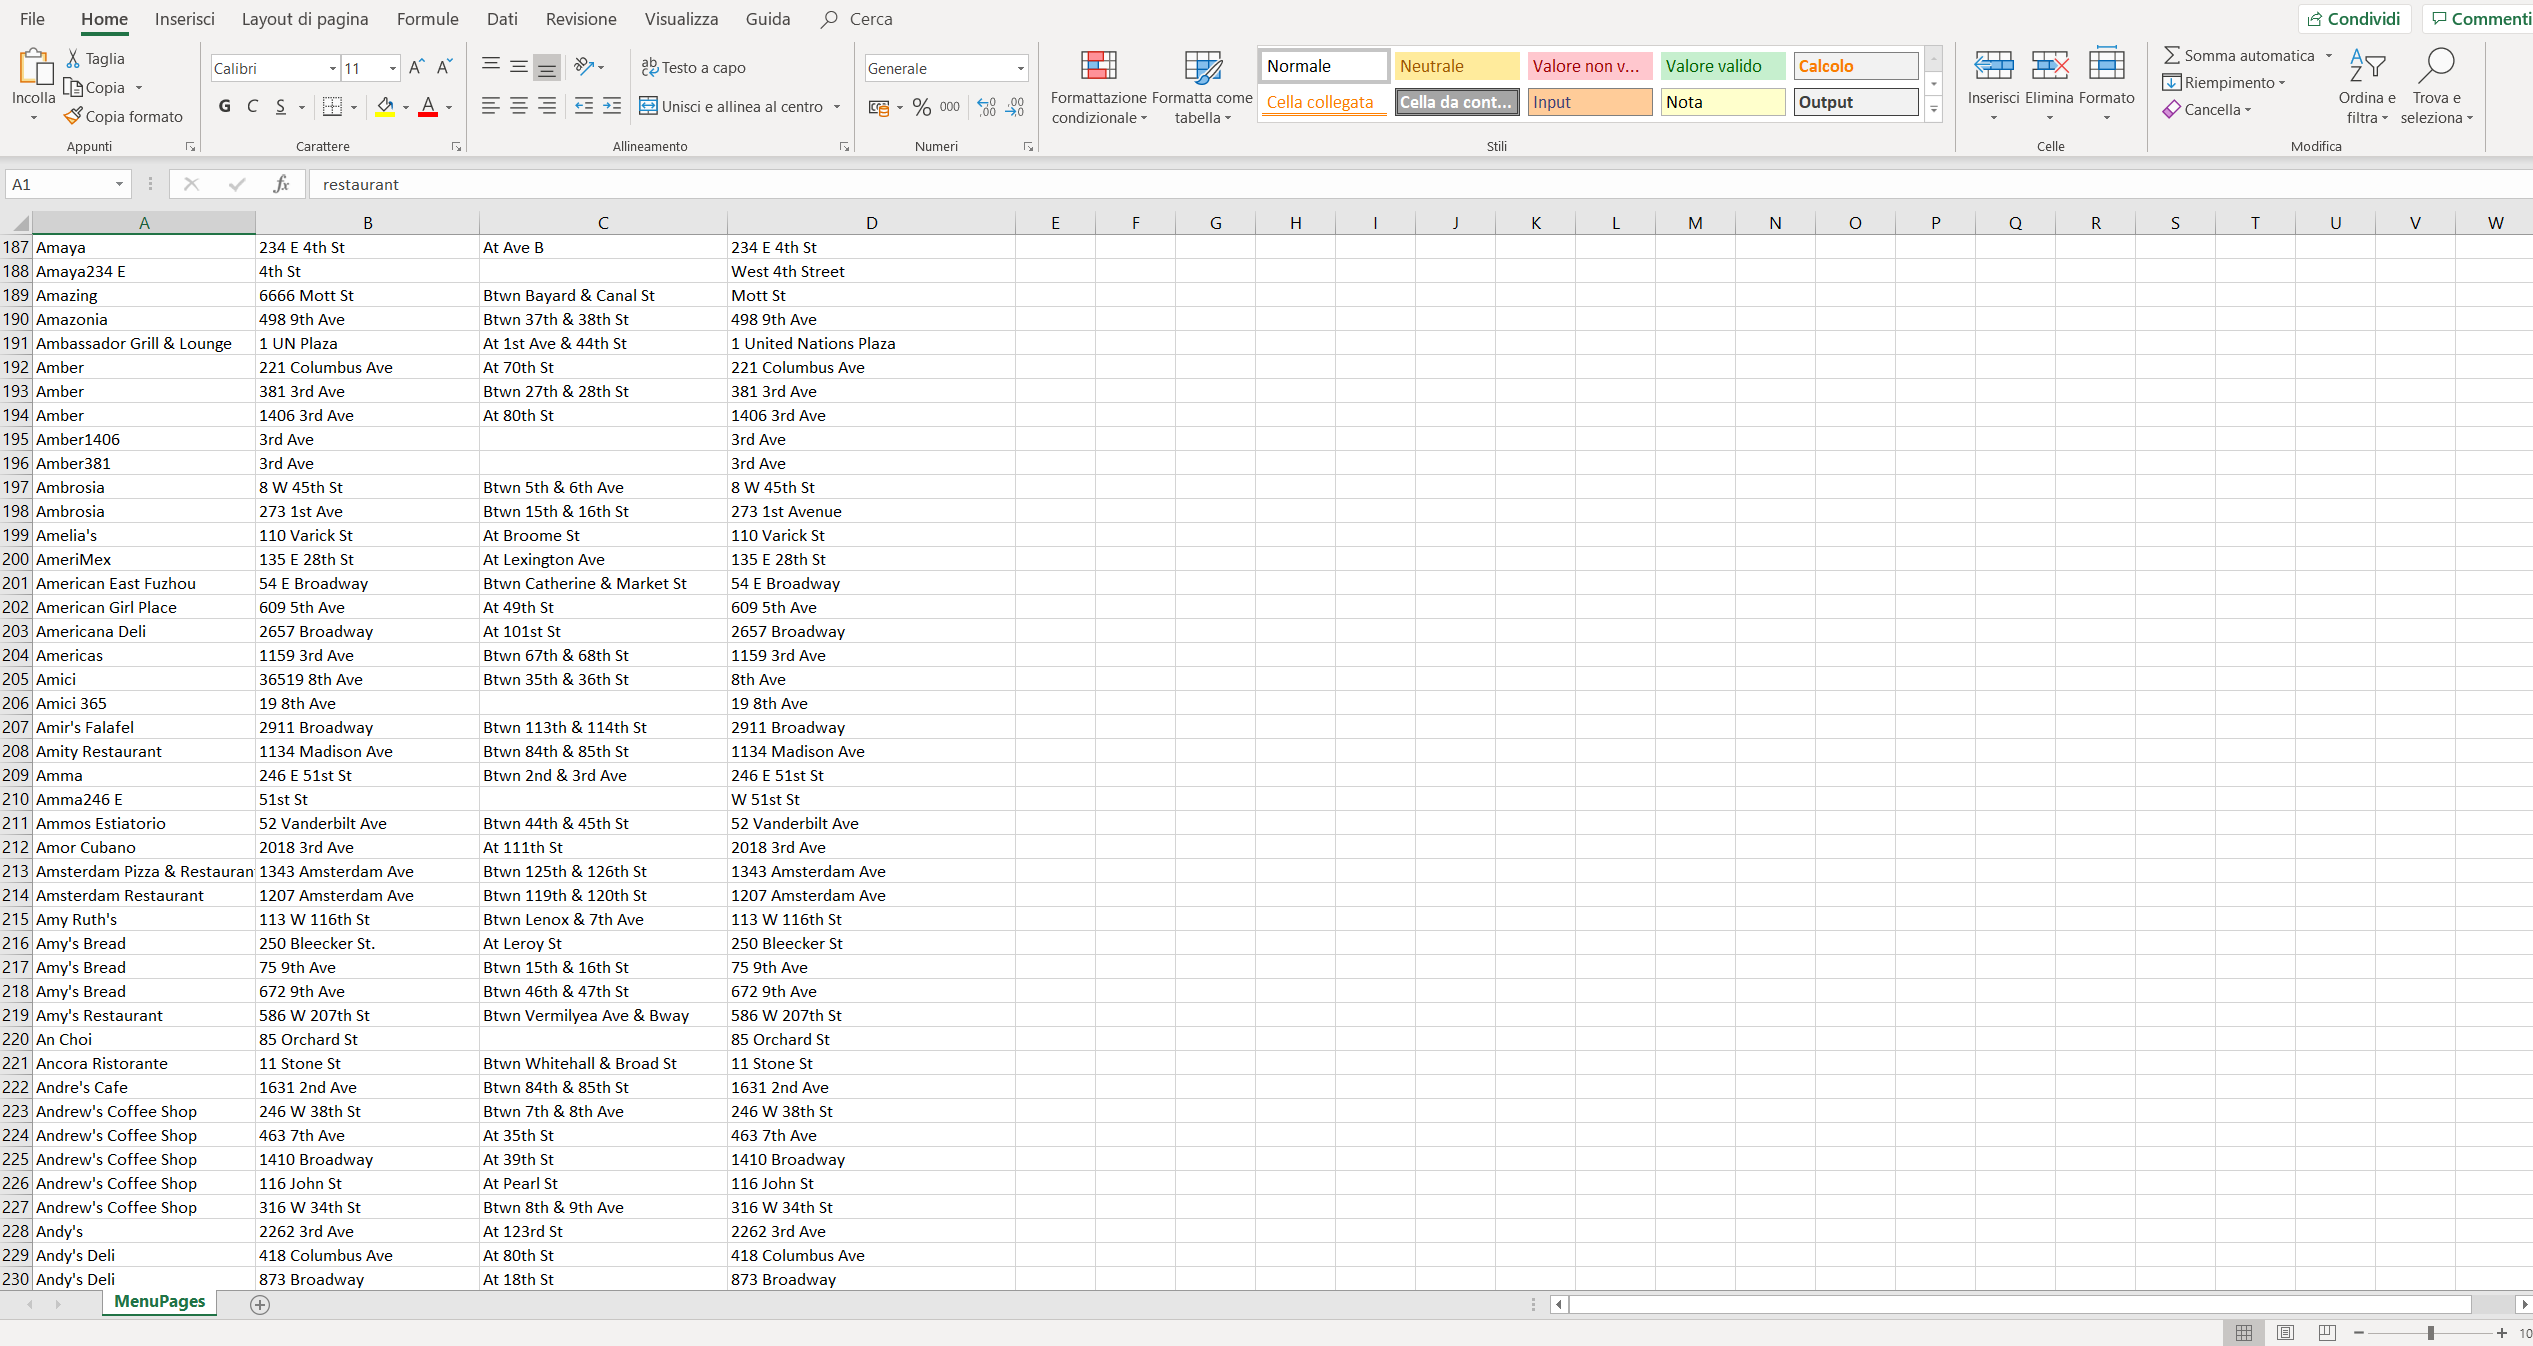
\includegraphics[width=0.9\linewidth]{img/new.png}
\caption{\textit{Dati dopo il preprocessing di MenuPages}}
\end{figure}

\newpage
\subsection{Record Linkage}
Dalla fase di preprocessing si ottengono in output 12 dataset, uno per ogni sito web presente nei file originali. Si deve affrontare dunque il problema di record linkage multiplo, che è stato affrontato con due approcci differenti, al fine di cercare di comprendere quale metodo sia migliore in termini di semplicità d'implementazione o di risultati ottenuti. I due approcci differiscono principalmente per la logica iniziale %%% da scrivere meglio non so come metterla giù

In entrambi i metodi, però, si seguono i passi principali del record linkage, che sono i seguenti:
\begin{itemize}
\item \textbf{Indexing} - permette di creare coppie di record, denominate \textit{candidate links}. Nel nostro algoritmo abbiamo implementato tre tecniche di indexing: \\
- \textit{full}, che crea le coppie effettuando il prodotto cartesiano dei due dataset, motivo per il quale è molto lungo e sconsigliato. \\
- \textit{blocking}, che permette di creare le coppie basandosi su una o più variabili uguali. \\
- \textit{sortedneighbourhood}, da usare nel momento in presenza di dataset con un grande numero di errori di spelling nei valori.
\item \textbf{Comparing} - viene usato per confrontare le coppie di record create nella fase di indexing, sfruttando diversi metodi di similarità. Nel nostro caso abbiamo effettuato un confronto fra stringhe testando alcuni dei vari metodi disponibili (‘jaro’, ‘jarowinkler’, ‘levenshtein’, ‘lcs’) e impostando un valore di soglia (tutti i confronti approssimativi di stringhe più alti o uguali a questa soglia valgono 1) oppure usato un confronto esatto nel momento in cui trattavamo l'attributo \textit{addressGoogle}, che sappiamo essere uniforme.
\item \textbf{Classification} - dove le coppie vengono classificate in matches, non-matches e possible matches. In particolare abbiamo deciso di applicare due algoritmi di apprendimento non supervisionato, non essendo in possesso di training data. Gli algoritmi adottati sono: \\
- \textit{ECM Classifier} o \textit{Expectation/Conditional Maxisation classifier}, un algoritmo probabilistico dove viene trovata iterativamente la massima probabilità (locale) o la massima stima a posteriori (MAP) dei parametri nei modelli statistici. L'iterazione EM si alterna tra l'esecuzione di un passaggio di aspettativa (E), che crea una funzione per l'aspettativa della verosimiglianza, e un passaggio di massimizzazione (M). \\
- \textit{KMeans Classifier}, algoritmo che suddivide le coppie di record in match e non-match ed ogni vettore di confronto appartiene al cluster con la media più vicina. L'algoritmo è calibrato per due cluster: un cluster di corrispondenza e un cluster di non corrispondenza.
\item {Evaluation} - permette di verificare la qualità del linkage in termini di accuratezza, recall e F-score. Purtroppo non ci è stato possibile eseguire questa fase in quanto sprovvisti di \textit{veri positivi}.
\end{itemize}


\subsubsection{Metodo 1}
%immagine
In questo approccio ci si è ricondotti al problema di record linkage fra due dataset passando dunque dai 12 dataset iniziali a due finali.

Analizzando i dataset ottenuti siamo riusciti ad individuare delle caratteristiche comuni in grado di distinguerli in due macro gruppi:
Nei dataset \textit{FoodBuzz, NYMag, NYTimes, OpenTable, SavoryCities} si hanno esclusivamente il nome del ristorante e il quartiere (solo in \textit{FoodBuzz} abbiamo in aggiunta l'indirizzo, che ci permetterà il linkage con l'altro dataset), nei dataset \textit{TimeOut, ActiveDiner, DiningGuide, MenuPages, TasteSpace, VillageVoice}, invece, abbiamo nome del ristorante e indirizzo in tutti i file.

\noindent Per ogni insieme di dataset, dopo aver uniformato i nomi e l'ordine delle colonne presenti, abbiamo eseguito un append di tutti i dataframe generati importando i file csv. 
Successivamente sono stati rimossi i duplicati presenti basandoci solo sulle colonne comuni per tutti, ossia \textit{restaurant} e \textit{neighbourhood} nel primo caso e \textit{restaurant} e \textit{addressGoogle} nel secondo.

\noindent Successivamente viene applicata la \textbf{deduplicazione}, ossia una tecnica usata per eliminare copie duplicate di dati ripetuti. È possibile applicarla sempre attraverso la libreria \textit{Record Linkage Toolkit} in quanto viene vista come un record linkage effettuato tra il database e se stesso. Come tecnica di \textit{indexing} usiamo \textit{sortedneighbourhood} ed effettuiamo la fase di \textit{comparing} sugli attributi comuni nei rispettivi gruppi di dataset.

\noindent In questa fase iniziale per classificare i match ci siamo basati esclusivamente sul punteggio di score ottenuto dalla fase di comparing, in modo da poter includere con sicurezza record che differivano solo di poche lettere (ad esempio i ristoranti "Bubba Gump Shrimp Co." e "Bubba Gump Shrimp Company"), scegliendo come valore di soglia dello score 1.75.

\noindent Una volta individuati i match sono stati unificati i dati in modo da creare un dataframe contenente le informazioni uniche utili per ogni match trovato. Per ottenere il dataset finale dal primo dataframe ottenuto come l'append dei csv importati sono state rimosse tutte le righe delle coppie presenti nei match e sono state aggiunti i record unificati contenenti le informazioni complete.

\noindent Da questa fase sono risultati due dataset, rispettivamente di 6468 e di 15093 record, invece dei 58614 record totali derivati dall'unione di tutti i 12 file iniziali.

\subsubsection{Metodo 2}
%CIAO FEDE TUTTO TUO 

\subsubsection{True Matches}
I dati di addestramento non sono generalmente disponibili nelle applicazioni di record linkage perché sono set di dati specifici del campione, infatti nel nostro caso non sono forniti dei true matches. \\

\noindent \textit{Python Record Linkage Toolkit}  fornisce un'interfaccia utente per la classificazione manuale delle coppie di record. Il software RecordLinkage Annotator utilizza un file di annotazione strutturato, che si può creare attraverso la funzione \href{https://recordlinkage.readthedocs.io/en/latest/annotation.html}{recordlinkage.write\_annotation\_file()} sia per il linkaggio che per la deduplicazione.\\
\begin{figure}[H]
	\centering
	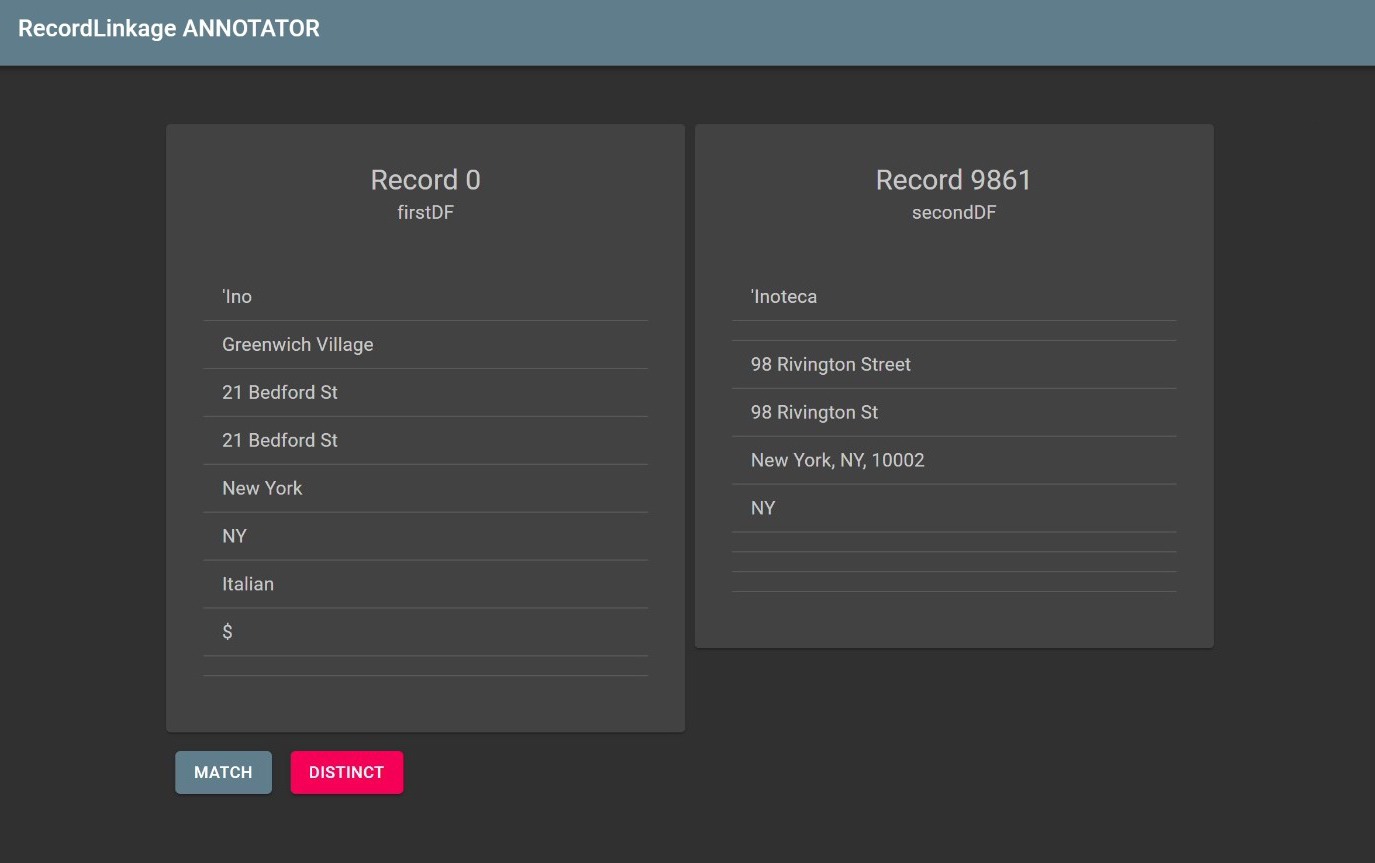
\includegraphics[width=0.8\linewidth]{img/matchCenter.png}
	\caption{\textit{Interfaccia web per la classificazione manuale}}
\end{figure}

Nel nostro caso abbiamo confrontato le prime 100 coppie derivate dalla fase di \textit{comparison}, ottenendo X match. Queste informazioni saranno fondamentali per poter valutare l'efficacia degli algoritmi di classificazione usati. 

\textbf{Risultati}: 
I dataset di partenza rappresentano un caso reale, siamo stati posti di fronte a dati inconsistenti, codificati in modi diversi, con attributi differenti e senza informazioni sui dati "veri" da poter usare come confronto per valutare l'efficacia del codice sviluppato, per questo possiamo analizzare in modo principalmente empirico i risultati ottenuti.

Grazie all'interfaccia fornita dalla libreria \textit{Record Linkage Toolkit} abbiamo generato un insieme di matches verificati manualmente su un insieme di 100 coppie, grazie ai quali possiamo valutare l'efficacia degli algoritmi di classificazione utilizzati su un sottoinsieme di 100 coppie individuate.

L'accuratezza dell'algoritmo ecm è 0.89 mentre di kmeans è 0.83
Abbiamo generato le seguenti matrici di confusione:
%come le riportiamo? 

Dopo aver individuato i match il dataset finale è dato dai record linkati (un record per coppia individuata) e i record per i quali non è stato individuato un match.
Con il primo metodo abbiamo ottenuto X record per il dataset generato dall'algoritmo ECM e X per il dataset generato dall'algoritmo Kmeans.


\newpage
\printbibliography[title=Bibliografia]

\end{document}
